\question
Для представленного графа и ДОПОЛНИТЕЛЬНОГО к нему выполните (в каждом) удаление не менее 3х ребер с сохранением связности графа. 
Для получившихся графов укажите: 
\begin{enumerate}
\item компоненты реберной двусвязности;
\item компоненты вершинной двусвзяности;
\item точки сочленения, если их нет, то укажите почему;
\item мосты, если их нет, то укажите почему;
\item Эйлеров цирк/цепь, если существует;
\item Гамильтонов цикл/цепь, если существует;
\end{enumerate}
\begin{figure}[h]

\begin{minipage}[h]{0.55\linewidth}
\end{minipage}
\begin{minipage}[h]{0.45\linewidth}
\center{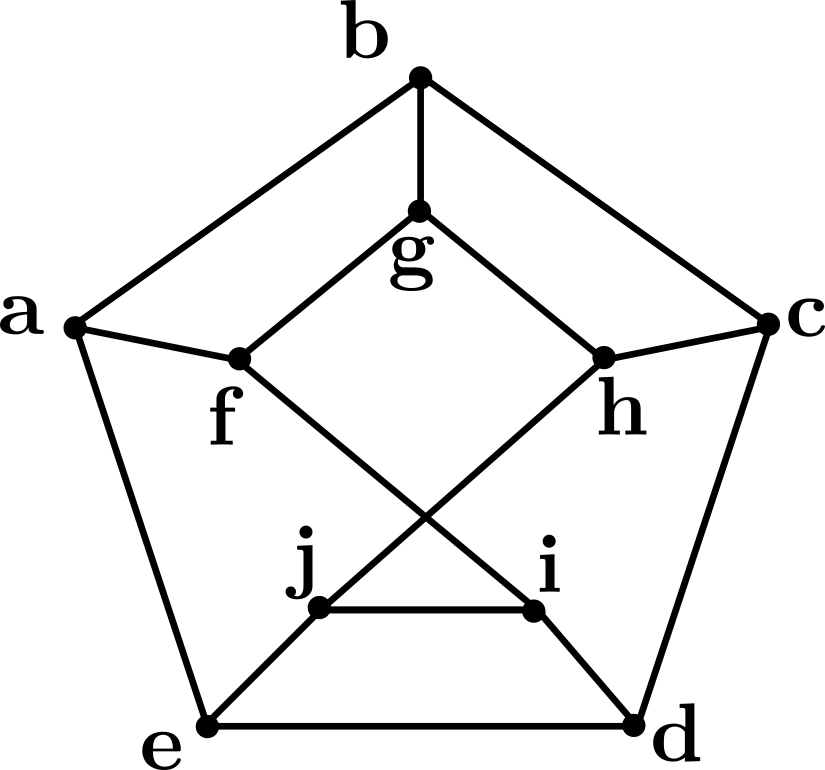
\includegraphics[width=0.45\textwidth]{pic/14.png} }
\end{minipage}
\end{figure}